\chapter{Equipment Health Assessment using Artificial Neural Networks}
%\chapter{Classification of Healthy and Faulty States using Neural Networks}

\chapterintrobox{This chapter demonstrates the use of an artificial neural network to estimate the health state of a set of turbofan engines from NASA C-MAPSS dataset and predict the remaining useful life. Also different metrics to assess the performance of the network will be introduced.}

\section{Introduction to NASA C-MAPSS dataset}
C-MAPSS is a tool for simulating a realistic large commercial turbofan engine. The software is coded in the MATLAB\textsuperscript{\textregistered} and Simulink\textsuperscript{\textregistered} environment. It includes a number of editable input parameters that allow the user to enter specific values of his/her own choice regarding operational profile, closed-loop controllers, environmental conditions, etc. \cite{Saxena2008}. 

\begin{wrapfigure}{r}{0.5\textwidth}
    \centering
    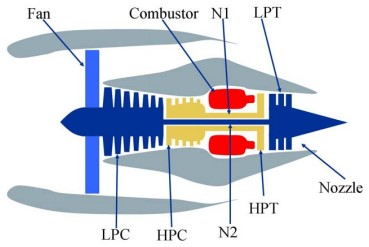
\includegraphics[width=.48\textwidth]{figures/c-mapss-engine-diagram.jpg}
    \caption{Simplified diagram of engine simulated in C-MAPSS \cite{Saxena2008}}
    \label{figure:c-mapss-engine-diagram}    
\end{wrapfigure}

Figure \ref{figure:c-mapss-engine-diagram} is a simplified diagram of the simulated engine showing its main elements, like low pressure compressor section (LPC), high pressure compressor section (HPC), fan and combustor. The dataset released by NASA Ames Research Center contains resulting data from simulating many turbofine engines, from beginning of operation until failure. The dataset was originally released for Prognostics and Health Management 2008 Data Competition, Table \ref{table:c-mapss-sensors} shows different variables, the output of the simulation and their units, that were provided for the participants in the competition:

\begin{table}[h]
    \centering
    \begin{tabular}{l|l|l}
        \hline
        \textbf{Symbol} & \textbf{Description} & \textbf{Units}\\
        \hline
        \textbf{T2} & Total temperature at fan inlet & R \\
        \textbf{T24} & Total temperature at LPC outlet & R \\
        \textbf{T30} & Total temperature at HPC outlet & R  \\
        \textbf{T50} &Total temperature at LPT & R\\
        \textbf{P2} & Pressure at fan inlet& psia\\
        \textbf{P15}& Total pressure in bypass-duct& psia\\
        \textbf{P30}& Total pressure at HPC outlet& psia\\
        \textbf{Nf}& Physical fan speed& rpm\\
        \textbf{Nc} & Physical core speed &rpm\\
        \textbf{epr}& Engine pressure ratio (P50/P2)& --\\
        \textbf{Ps30}& Static pressure at HPC outlet& psia\\
        \textbf{phi}& Ratio of fuel flow to Ps30& pps/psi\\
        \textbf{NRf}& Corrected fan speed &rpm\\
        \textbf{NRc}& Corrected core speed& rpm\\
        \textbf{BPR}& Bypass Ratio& --\\
        \textbf{farB}& Burner fuel-air ratio &--\\
        \textbf{htBleed}& Bleed Enthalpy &-- \\
        \textbf{Nf\_dmd} &Demanded fan speed& rpm\\
        \textbf{PCNfR\_dmd}& Demanded corrected fan speed &rpm\\
        \textbf{W31} & HPT coolant bleed & lbm/s \\
        \textbf{W32} & LPT coolant bleed & lbm/ \\
        \hline
    \end{tabular}
    \caption{C-MAPSS outputs to measure system response.}
    \label{table:c-mapss-sensors}
\end{table}

\section{Visualization of equipment degredation}
Visualizing the simulation output can give a sense of how these variables change during the life of the engine, Figure \ref{fig:sensors-plot} shows four different sensors from one of the engines (values are normalized):

\begin{figure}[ht]
    \centering
    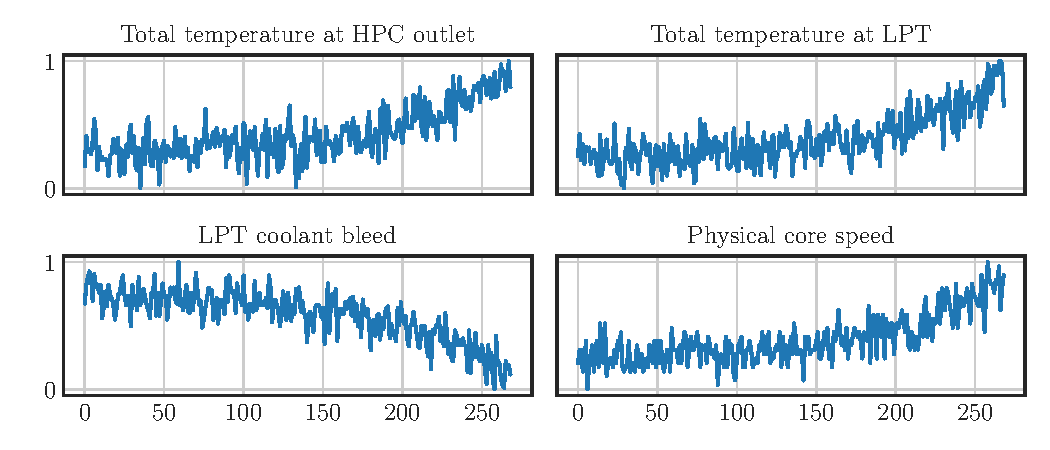
\includegraphics[width=\linewidth]{figures/plots/sensors_plot.pdf}
    \caption{Development of 6 sensors outputs from one of the engines (normalized)}
    \label{fig:sensors-plot}
\end{figure}

It is apparent that sensors output follow a specific pattern (increasing or decreasing) from beginning of operation until breakdown, this is very useful and can increase the robustness of the predictive model.

Alternatively, all sensors values can be combined and visualized altogether using Principal Component Analysis (section \ref{section:dimensionality-reduction}) to reveal the general trend in the data a dimsneionality reduction technique, if condition monitoring data is directly indicative of the equipment health state, visualization of principal components can show apparent visual degradation patterns.

\begin{figure}[ht]
    \centering
    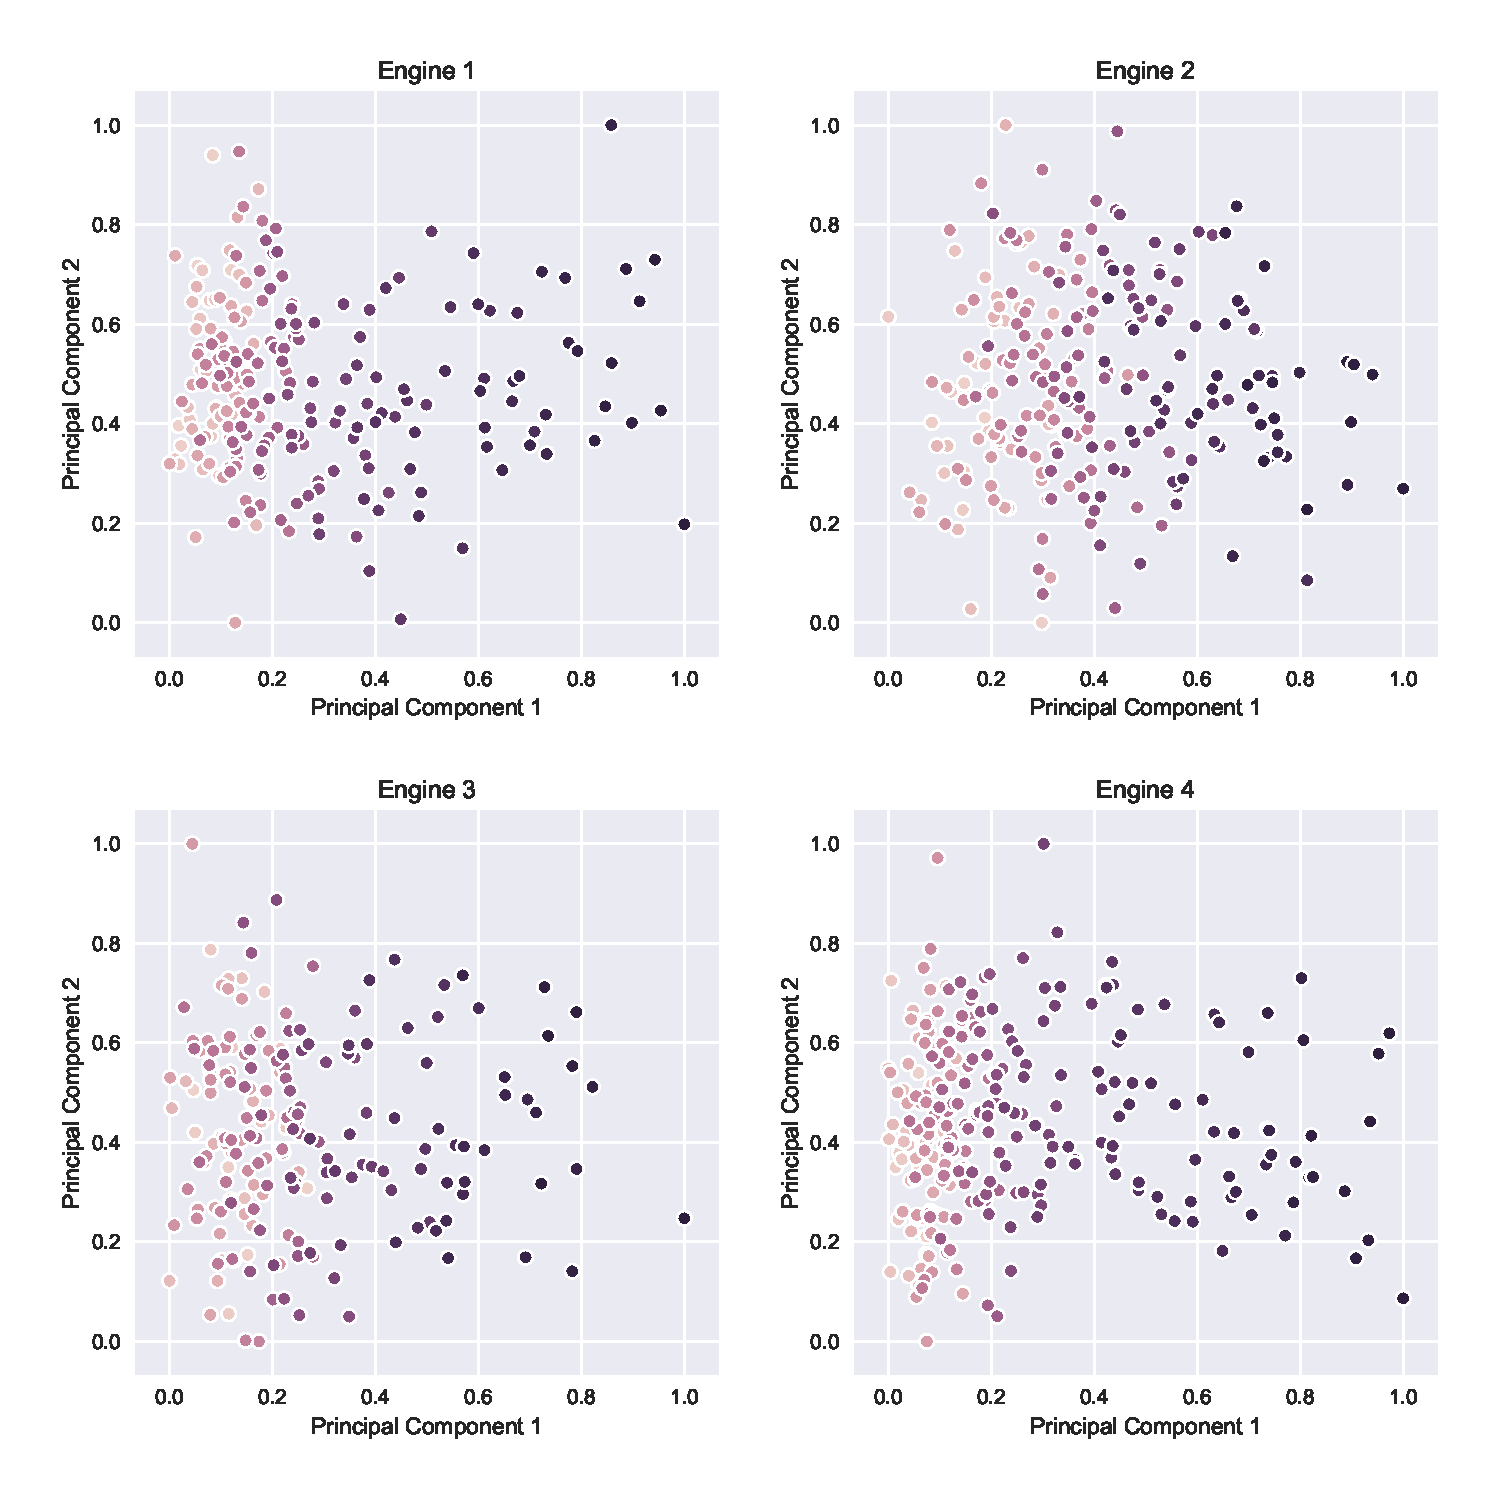
\includegraphics[width=.9\linewidth]{figures/plots/pc-degradation.pdf}
    \caption{Equipment health degredation (darkening color indicates advancing of health degradation) of four turbofan engines from C-MAPSS dataset}
    \label{fig:pca-degradation}
\end{figure}

Sensors values from 4 different engines are combined using PCA and the two first principal components are represented on Figure \ref{fig:pca-degradation}. There is absolutely an apparent pattern for health state degradation across the different engines from left (where lighter colors indicate normal working state) to the right (where the darkening color indicates fault development).

\section{Conclusion}
% TODO: translate
Fully-connected neural networks are a powerful tool for quantifying health state of complex systems using condition monitoring data. C-MAPSS dataset is an example of a system with many interacting parts that provide a variety of condition-monitoring data (e.g. temperature, pressure, rpm, …) where the degradation isn't directly related to one component but is indicated by the sum of the trends in all the monitoring data. Neural networks are able to capture such trends and produce a mapping from this data to the actual health of the machine.